\section{Low-Level Concepts}\label{sec:lowlevel}

\subsection{UML Diagrams}\label{subsec:umldiagrams}
\subsubsection{Component Diagram}\label{subsubsec:component}
Component diagram of my prototype is given in Figure~\ref{fig:Component_Diagram}.
\begin{figure}
	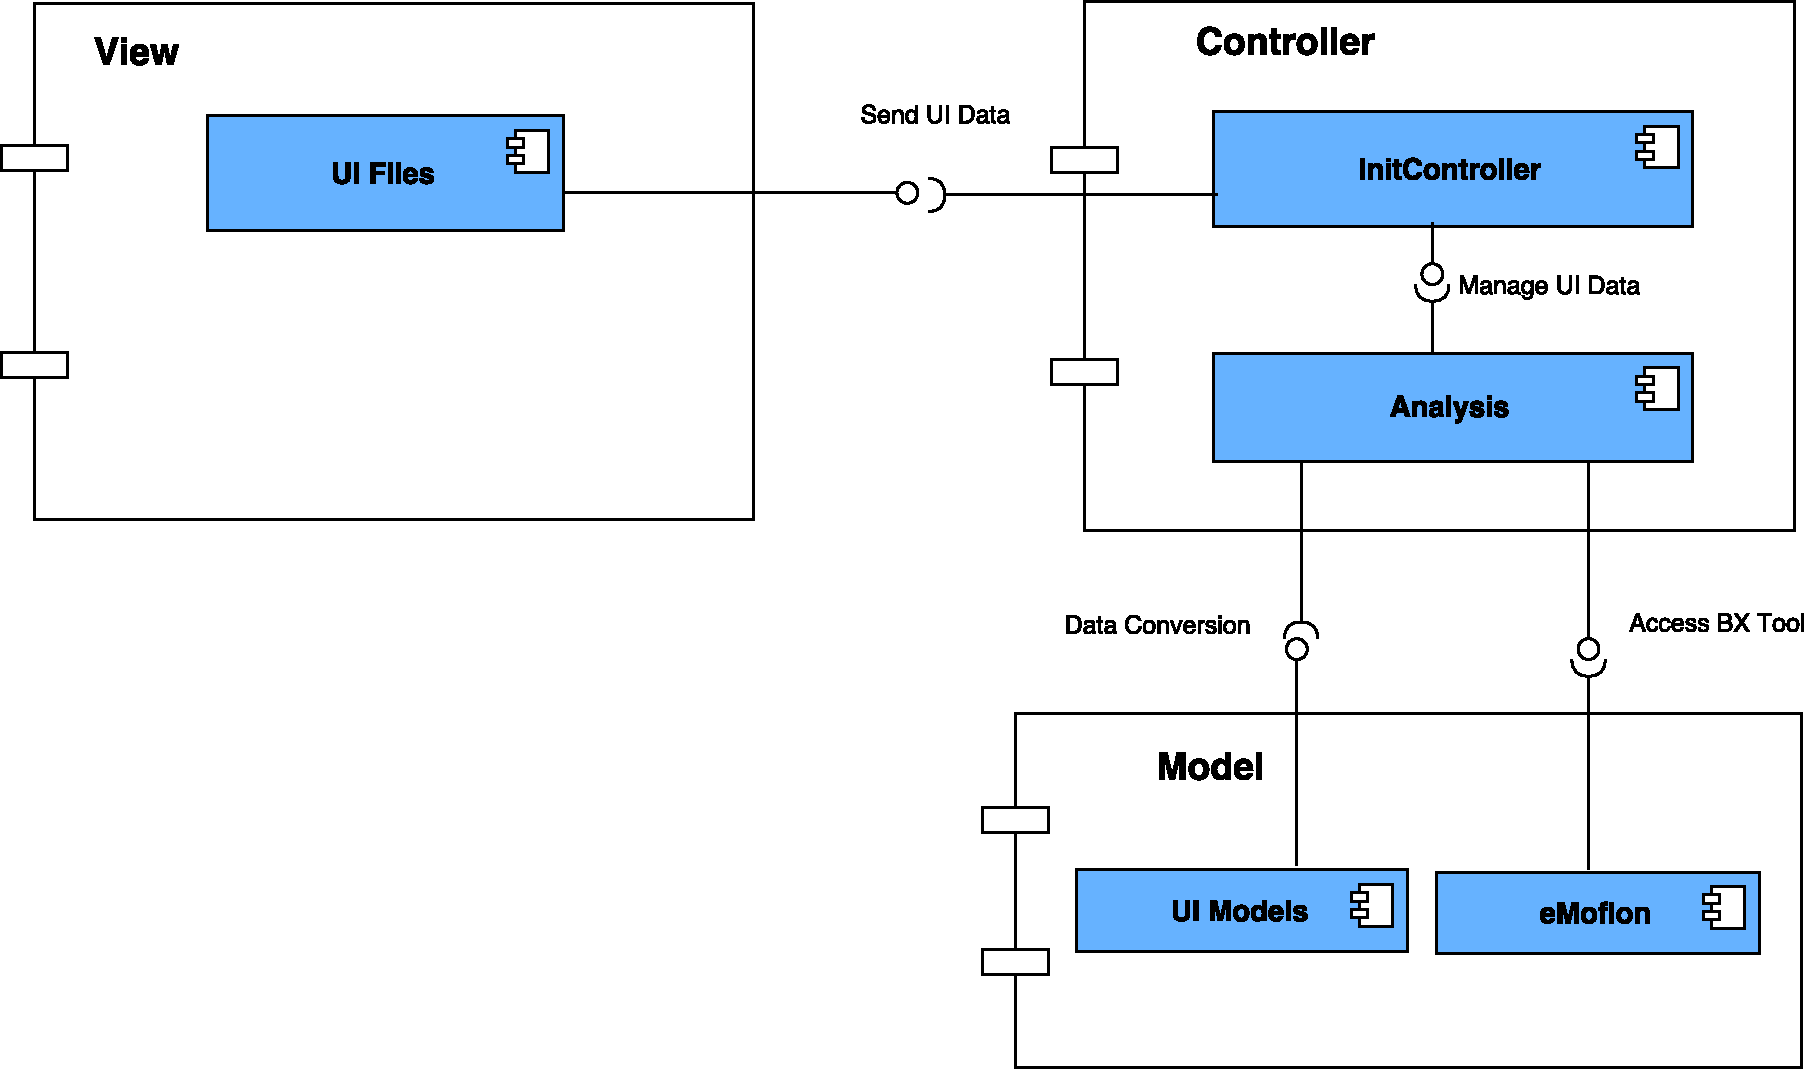
\includegraphics[width=1\textwidth]{figures/Component_Diagram}
	\caption{Component Diagram}
	\label{fig:Component_Diagram}
\end{figure}

I am using Model-View-Controller (MVC) pattern for my application framework. 
On the top, \texttt{View} (Web Browser) component is present which contains a graphical user interface and functionalities that belong to the user. With the changes on \texttt{View} component, data are being provided through interface \texttt{IDoAnalysis} to the \texttt{Controller} component and after the calculations are done, the results are sent back to the \texttt{View} through interface \texttt{IProvideResults}. Both \texttt{View} and \texttt{Controller} resides on the same machine. \texttt{Model} (Bx Tool) component encapsulates and manages the state of all models by communication with the \texttt{Controller} through interface \texttt{IRules}.
\subsubsection{Class Diagram}\label{subsubsec:classes}
\subsubsection{Sequence Diagram}\label{subsubsec:sequence}

\subsection{Core Details}\label{subsec:coredetails}

 



